% Human Activity Recognition Using Wearable Sensors — CVPR Format Report
% Authors: Sourabh Singh, Ranvir Singh | IIT Jodhpur | November 2026
\documentclass[10pt,twocolumn,letterpaper]{article}

\usepackage{cvpr}
\usepackage{times}
\usepackage{graphicx}
\usepackage{amsmath}
\usepackage{amssymb}
\usepackage{booktabs}
\usepackage{hyperref}
\usepackage{float}

\begin{document}

\title{Human Activity Recognition Using Wearable Sensors}

\author{
Sourabh Singh (M25CPS009) \quad Ranvir Singh (P25CS0007)\\
Indian Institute of Technology Jodhpur\\
{\tt\small m25cps009@iitj.ac.in, p25cs0007@iitj.ac.in}\\[6pt]
{\small Repository: \url{https://github.com/Sourabh16/Human-Activity-Recognition-Using-Wearable-Sensors}}\\
{\small Final Commit: \texttt{f87cb5e} $\mid$ November 27, 2026}
}

\maketitle

% ═══════════════════════════════════════════════
\begin{abstract}
This report presents a complete machine learning pipeline for Human Activity Recognition (HAR) using the MHEALTH wearable sensor dataset. We employ a Support Vector Classifier (SVC) with a Radial Basis Function (RBF) kernel, leveraging the kernel trick to construct non-linear decision boundaries in a high-dimensional feature space. From 21 motion sensor channels sampled at 50~Hz, we extract 273 time-domain and frequency-domain features using sliding window segmentation. The model, optimized via GridSearchCV with SMOTE-based class balancing, achieves a test accuracy of \textbf{94.92\%} under a rigorous subject-independent evaluation protocol. A subsequent sensor-location ablation study reveals that removing ankle sensor features \textit{improves} generalization by 1.11\%, exposing inter-sensor redundancy. PCA-based correlation analysis confirms high multicollinearity between ankle features and those from chest and arm sensors. These findings underscore that careful feature and sensor selection remain critical even when non-linear kernel methods are used.
\end{abstract}

% ═══════════════════════════════════════════════
\section{Introduction}

Human Activity Recognition (HAR) is a fundamental problem in ubiquitous computing, with applications spanning healthcare monitoring, elderly fall detection, sports analytics, and context-aware mobile systems~\cite{bulling2014tutorial}. The goal is to classify a person's physical activity (e.g., walking, running, sitting) from time-series data captured by wearable inertial sensors.

Traditional approaches to HAR rely on handcrafted features extracted from accelerometer, gyroscope, and magnetometer signals, followed by classical machine learning classifiers. While deep learning methods have recently gained popularity for HAR tasks~\cite{ordonez2016deep, khatun2022deep}, Support Vector Machines (SVMs) remain a compelling choice due to their strong theoretical foundations, excellent performance in high-dimensional spaces, and interpretability~\cite{vapnik1995nature}.

The \textbf{kernel trick}~\cite{scholkopf2002learning} is central to SVM's effectiveness: it allows the classifier to operate in an implicitly mapped high-dimensional (potentially infinite-dimensional) feature space without explicitly computing the transformation. The RBF kernel $K(x_i, x_j) = \exp(-\gamma \|x_i - x_j\|^2)$ is particularly effective for HAR because activity boundaries in sensor feature space are inherently non-linear --- static postures like standing and sitting produce nearly identical accelerometer means but differ in subtle distributional properties.

This work makes the following contributions:
\begin{enumerate}
    \item A complete, reproducible HAR pipeline achieving \textbf{94.92\%} test accuracy on the MHEALTH dataset with subject-independent evaluation.
    \item Comprehensive feature engineering: 13 time-domain and frequency-domain features per sensor channel, yielding 273 features per 5.12-second window.
    \item A sensor-location ablation study revealing that ankle sensor features introduce redundancy that \textit{degrades} generalization, with PCA-based evidence of inter-sensor multicollinearity.
    \item All code, instructions, and reproducibility artifacts are publicly available.\footnote{\url{https://github.com/Sourabh16/Human-Activity-Recognition-Using-Wearable-Sensors}}
\end{enumerate}

% ═══════════════════════════════════════════════
\section{Related Work}

\subsection{HAR with Classical Methods}
Early HAR systems used statistical features with classifiers such as Decision Trees, Naive Bayes, and SVMs~\cite{bao2004activity}. Bao and Intille~\cite{bao2004activity} were among the first to demonstrate that body-worn accelerometers combined with simple decision-tree classifiers could recognise everyday activities with reasonable accuracy. Anguita et al.~\cite{anguita2013public} later demonstrated competitive results using SVMs on smartphone accelerometer data, establishing SVMs as a strong baseline for sensor-based HAR. The key advantage of these approaches is their interpretability and low computational cost, making them suitable for deployment on resource-constrained wearable devices.

The choice of features has been shown to matter more than the choice of classifier in many HAR studies~\cite{bulling2014tutorial}. Time-domain features such as mean, variance, and zero-crossing rate capture the overall shape and intensity of movement, while frequency-domain features derived from FFT and power spectral density capture periodicity --- a critical discriminator between rhythmic activities like walking and jogging. Our work builds on this tradition by extracting a comprehensive 13-feature set per channel that spans both domains.

\subsection{SVM Theory and the Kernel Trick}
The SVM was introduced by Cortes and Vapnik~\cite{cortes1995support} as a maximum-margin classifier. For linearly separable data, the SVM finds the hyperplane that maximises the geometric margin between classes, providing strong generalisation guarantees rooted in VC dimension theory~\cite{vapnik1995nature}. For non-linearly separable data, the kernel trick~\cite{scholkopf2002learning} enables the SVM to operate in an implicitly mapped high-dimensional feature space $\mathcal{H}$ by replacing all inner products $\langle \phi(x_i), \phi(x_j) \rangle$ with a kernel function $K(x_i, x_j)$. The RBF kernel $K(x_i, x_j) = \exp(-\gamma\|x_i - x_j\|^2)$ corresponds to an infinite-dimensional $\mathcal{H}$ (via its Taylor series expansion), giving the SVM maximal flexibility while remaining computationally tractable.

This theoretical elegance makes SVM with the RBF kernel particularly well-suited for HAR: the 273-dimensional feature space we construct contains non-linear class boundaries (e.g., standing vs.\ sitting differ in subtle distributional moments, not in means), and the kernel trick handles these without explicit feature engineering beyond our initial extraction step.

\subsection{Deep Learning Approaches}
Ord{\'o}{\~n}ez and Roggen~\cite{ordonez2016deep} applied deep CNNs and LSTMs to multimodal wearable data, achieving 91\% accuracy on MHEALTH by learning features directly from raw sensor streams. Khatun et al.~\cite{khatun2022deep} combined CNN-LSTM with self-attention mechanisms to reach 98.76\% accuracy. While these results are impressive, they come with significant costs: deep models require GPUs for training, need substantially more data to avoid overfitting, and produce opaque, non-interpretable internal representations. For applications in clinical settings or safety-critical systems, the interpretability of handcrafted features and classical classifiers remains a significant advantage.

\subsection{The MHEALTH Dataset}
The MHEALTH dataset~\cite{banos2014mhealthdroid} has been widely adopted as a benchmark for HAR research. It offers multi-sensor, multi-subject data with clearly defined activity labels, enabling rigorous evaluation under subject-independent protocols. The dataset's inclusion of sensors at three distinct body locations (chest, ankle, arm) makes it particularly suitable for studying sensor placement strategies and inter-sensor redundancy --- a known concern in multi-sensor HAR systems~\cite{bulling2014tutorial} that we investigate through our ablation study.

% ═══════════════════════════════════════════════
\section{Dataset}

\subsection{Overview}
The MHEALTH (Mobile Health) dataset~\cite{banos2014mhealthdroid} comprises data from 10 volunteers performing 12 physical activities. Three Shimmer wearable sensors were placed on the \textbf{chest}, \textbf{left ankle}, and \textbf{right wrist/arm}. Each sensor captures tri-axial acceleration; the ankle and arm sensors additionally record gyroscope and magnetometer readings. A two-lead ECG is recorded from the chest. All signals are sampled at 50~Hz.

\subsection{Activity Classes}
The 12 activities span a range of motion intensities, from static postures (standing, sitting, lying down) to moderate activities (walking, cycling) and vigorous movements (jogging, running, jumping). The null class (label 0), representing transition periods, is excluded during preprocessing.

\subsection{Data Statistics}
Table~\ref{tab:dataset} summarises the dataset composition. The total dataset contains 1,215,745 sensor readings across all subjects.

\begin{table}[H]
\centering
\caption{MHEALTH dataset statistics per subject.}
\label{tab:dataset}
\small
\begin{tabular}{lrr}
\toprule
\textbf{Subject} & \textbf{Total Rows} & \textbf{Split} \\
\midrule
Subject 1  & 161,280 & Train \\
Subject 2  & 130,561 & Train \\
Subject 3  & 122,112 & Train \\
Subject 4  & 116,736 & Train \\
Subject 5  & 119,808 & Train \\
Subject 6  & 98,304  & Train \\
Subject 7  & 104,448 & Train \\
\midrule
Subject 8  & 129,024 & Test \\
Subject 9  & 135,168 & Test \\
Subject 10 & 98,304  & Test \\
\midrule
\textbf{Total} & \textbf{1,215,745} & --- \\
\bottomrule
\end{tabular}
\end{table}

\subsection{Sensor Configuration}
Table~\ref{tab:sensors} details the sensor channels used after preprocessing (ECG columns are dropped).

\begin{table}[H]
\centering
\caption{Sensor channels used for classification (21 total).}
\label{tab:sensors}
\small
\begin{tabular}{llc}
\toprule
\textbf{Location} & \textbf{Sensor} & \textbf{Channels} \\
\midrule
Chest      & Accelerometer       & 3 \\
Left Ankle & Accelerometer       & 3 \\
Left Ankle & Gyroscope           & 3 \\
Left Ankle & Magnetometer        & 3 \\
Right Arm  & Accelerometer       & 3 \\
Right Arm  & Gyroscope           & 3 \\
Right Arm  & Magnetometer        & 3 \\
\midrule
\multicolumn{2}{l}{\textbf{Total}} & \textbf{21} \\
\bottomrule
\end{tabular}
\end{table}

% ═══════════════════════════════════════════════
\section{Methodology}

\subsection{Preprocessing}
Raw sensor readings are cleaned through three steps: (1)~removal of null-class rows (label~0), which eliminates 611,430 of 853,249 training samples; (2)~exclusion of ECG columns, which are physiological rather than motion-related; and (3)~forward-fill imputation of any missing values. Features are then standardised using Z-score normalisation (zero mean, unit variance) fitted exclusively on training data to prevent data leakage.

\subsection{Sliding Window Segmentation}
The continuous time-series is segmented into fixed-length windows of 256 samples (5.12 seconds at 50~Hz) with 50\% overlap (step size = 128 samples). Windows are extracted per-subject to prevent cross-subject contamination. Each window receives the \textbf{mode label} (most frequent activity label within the window). This yields 1,879 training windows (Subjects 1--7) and 788 test windows (Subjects 8--10).

\subsection{Feature Engineering}
From each of the 21 sensor channels in each window, we extract 13 features spanning time-domain and frequency-domain representations, as detailed in Table~\ref{tab:features}. This produces a feature vector of dimensionality $21 \times 13 = 273$ per window.

\begin{table}[H]
\centering
\caption{Extracted features per sensor channel (13 total).}
\label{tab:features}
\small
\begin{tabular}{llp{3.8cm}}
\toprule
\textbf{Feature} & \textbf{Domain} & \textbf{Formula / Description} \\
\midrule
Mean        & Time & $\bar{x} = \frac{1}{N}\sum x_i$ \\
Std Dev     & Time & $\sigma = \sqrt{\frac{1}{N}\sum(x_i - \bar{x})^2}$ \\
Min         & Time & $\min(x)$ \\
Max         & Time & $\max(x)$ \\
Range       & Time & $\max(x) - \min(x)$ \\
Skewness    & Time & Third standardised moment \\
Kurtosis    & Time & Fourth standardised moment \\
RMS         & Time & $\sqrt{\frac{1}{N}\sum x_i^2}$ \\
ZCR         & Time & $\frac{1}{N}\sum \mathbb{1}[x_i x_{i+1} < 0]$ \\
\midrule
Dom.\ Freq. & Freq & $\arg\max_f |X(f)|^2$ via FFT \\
PSD Mean    & Freq & Mean of Welch PSD \\
PSD Peak    & Freq & Max of Welch PSD \\
Energy      & Freq & $\frac{1}{N}\sum x_i^2$ \\
\bottomrule
\end{tabular}
\end{table}

\subsection{Class Balancing with SMOTE}
The training set exhibits class imbalance: ``Jump front \& back'' has only 54 windows versus $\sim$200 for ``Standing still''. We apply SMOTE (Synthetic Minority Over-sampling Technique)~\cite{chawla2002smote} with $k=5$ nearest neighbours to generate synthetic minority samples by linear interpolation in feature space. This increases the training set from 1,879 to 2,052 balanced samples. Additionally, we set \texttt{class\_weight=`balanced'} in the SVC to further adjust for residual imbalance.

\subsection{SVM with RBF Kernel}
We use a Support Vector Classifier with the RBF kernel:
\begin{equation}
K(x_i, x_j) = \exp\left(-\gamma \|x_i - x_j\|^2\right)
\end{equation}
The RBF kernel implicitly maps inputs to an infinite-dimensional Hilbert space via its Taylor expansion, allowing the SVM to learn arbitrarily complex decision boundaries. The decision function for a test point $x$ is:
\begin{equation}
f(x) = \text{sign}\left(\sum_{i \in \mathcal{SV}} \alpha_i y_i K(x, x_i) + b\right)
\end{equation}
where $\mathcal{SV}$ denotes the set of support vectors, $\alpha_i$ are dual coefficients, and $b$ is the bias term.

\subsection{Hyperparameter Optimisation}
We perform an exhaustive grid search over the parameter space shown in Table~\ref{tab:grid}, evaluated with 5-fold stratified cross-validation (12 candidates $\times$ 5 folds = 60 fits).

\begin{table}[H]
\centering
\caption{GridSearchCV parameter space.}
\label{tab:grid}
\small
\begin{tabular}{ll}
\toprule
\textbf{Parameter} & \textbf{Values} \\
\midrule
$C$ (regularisation) & 0.1, 1, 10 \\
Kernel & RBF, Polynomial \\
$\gamma$ & scale, auto \\
\bottomrule
\end{tabular}
\end{table}

The regularisation parameter $C$ controls the trade-off between margin width and training error. Higher $C$ values penalise misclassifications more aggressively. The $\gamma$ parameter determines the influence radius of each support vector: $\gamma_{\text{scale}} = 1 / (n_{\text{features}} \cdot \text{Var}(X))$ adapts to the data dimensionality and variance.

% ═══════════════════════════════════════════════
\section{Results}

\subsection{Model Selection}
GridSearchCV identified the optimal configuration as $C=10$, kernel=RBF, $\gamma=\text{scale}$. Table~\ref{tab:model_summary} presents the complete model performance summary.

\begin{table}[H]
\centering
\caption{Summary of model selection and performance.}
\label{tab:model_summary}
\small
\begin{tabular}{lr}
\toprule
\textbf{Metric} & \textbf{Value} \\
\midrule
Best $C$ & 10 \\
Best kernel & RBF \\
Best $\gamma$ & scale \\
GridSearch candidates & 12 \\
Total CV fits & 60 \\
\midrule
Train accuracy (SMOTE) & 100.00\% \\
Mean CV accuracy & 95.13\% $\pm$ 0.66\% \\
\textbf{Test accuracy} & \textbf{94.92\%} \\
\bottomrule
\end{tabular}
\end{table}

The negligible gap between CV accuracy (95.13\%) and test accuracy (94.92\%) confirms that the model generalises well and is not overfitting despite the perfect training accuracy (which is expected on SMOTE-augmented data, where the synthetic interpolated points are easily fit by the RBF kernel).

The choice of $C=10$ over $C=0.1$ or $C=1$ indicates that the data benefits from a tighter fit: the 273 features we engineered are clean and discriminative enough that the SVM can aggressively fit without overfitting. The preference for $\gamma=\text{scale}$ (which sets $\gamma = 1/(273 \cdot \text{Var}(X))$) over $\gamma=\text{auto}$ ($1/273$) shows that accounting for feature variance improves the kernel's similarity metric.

\subsection{Per-Class Performance}
Table~\ref{tab:results} presents the full classification report. Several observations emerge:

\begin{table}[H]
\centering
\caption{Classification report on the test set (Subjects 8--10).}
\label{tab:results}
\small
\begin{tabular}{lcccc}
\toprule
\textbf{Activity} & \textbf{P} & \textbf{R} & \textbf{F1} & \textbf{N} \\
\midrule
Standing still       & 0.90 & 0.88 & 0.89 & 73 \\
Sitting \& relaxing  & 0.88 & 0.95 & 0.91 & 73 \\
Lying down           & 1.00 & 1.00 & 1.00 & 71 \\
Walking              & 0.91 & 1.00 & 0.95 & 72 \\
Climbing stairs      & 0.97 & 0.90 & 0.93 & 70 \\
Waist bends fwd      & 0.98 & 1.00 & 0.99 & 57 \\
Frontal elev.\ arms  & 0.98 & 0.96 & 0.97 & 67 \\
Knees bending        & 0.87 & 0.98 & 0.92 & 66 \\
Cycling              & 0.97 & 0.83 & 0.90 & 72 \\
Jogging              & 1.00 & 0.97 & 0.99 & 72 \\
Running              & 0.99 & 0.99 & 0.99 & 72 \\
Jump front \& back   & 1.00 & 0.96 & 0.98 & 23 \\
\midrule
\textbf{Weighted Avg} & \textbf{0.95} & \textbf{0.95} & \textbf{0.95} & 788 \\
\bottomrule
\end{tabular}
\end{table}

\textbf{Static activities:} ``Lying down'' achieves perfect classification (F1~=~1.00), as the supine posture produces a distinctive gravity-axis signature. ``Standing still'' and ``Sitting and relaxing'' show slight mutual confusion (precision 0.88--0.90), which is expected since both are low-motion postures differing primarily in trunk angle.

\textbf{Locomotion:} ``Walking'' (F1~=~0.95), ``Jogging'' (F1~=~0.99), and ``Running'' (F1~=~0.99) are well-separated due to their distinct step frequencies and acceleration magnitudes. The FFT dominant frequency feature is particularly discriminative here.

\textbf{Cycling:} This activity has the lowest recall (0.83), likely because the seated cycling posture shares trunk-level sensor patterns with stationary activities, while the leg motion is primarily captured by the ankle sensor.

\textbf{Exercises:} ``Waist bends forward'' (F1~=~0.99) and ``Frontal elevation of arms'' (F1~=~0.97) are captured well by arm and chest sensors respectively. ``Knees bending'' achieves high recall (0.98) but lower precision (0.87), suggesting some other activities are occasionally misclassified as crouching.

\subsection{Confusion Matrix}
Figure~\ref{fig:cm} shows the normalised confusion matrix. The strong diagonal confirms high per-class accuracy. Off-diagonal entries reveal the main confusion pairs: standing$\leftrightarrow$sitting and cycling$\leftrightarrow$climbing stairs.

\begin{figure}[H]
\centering
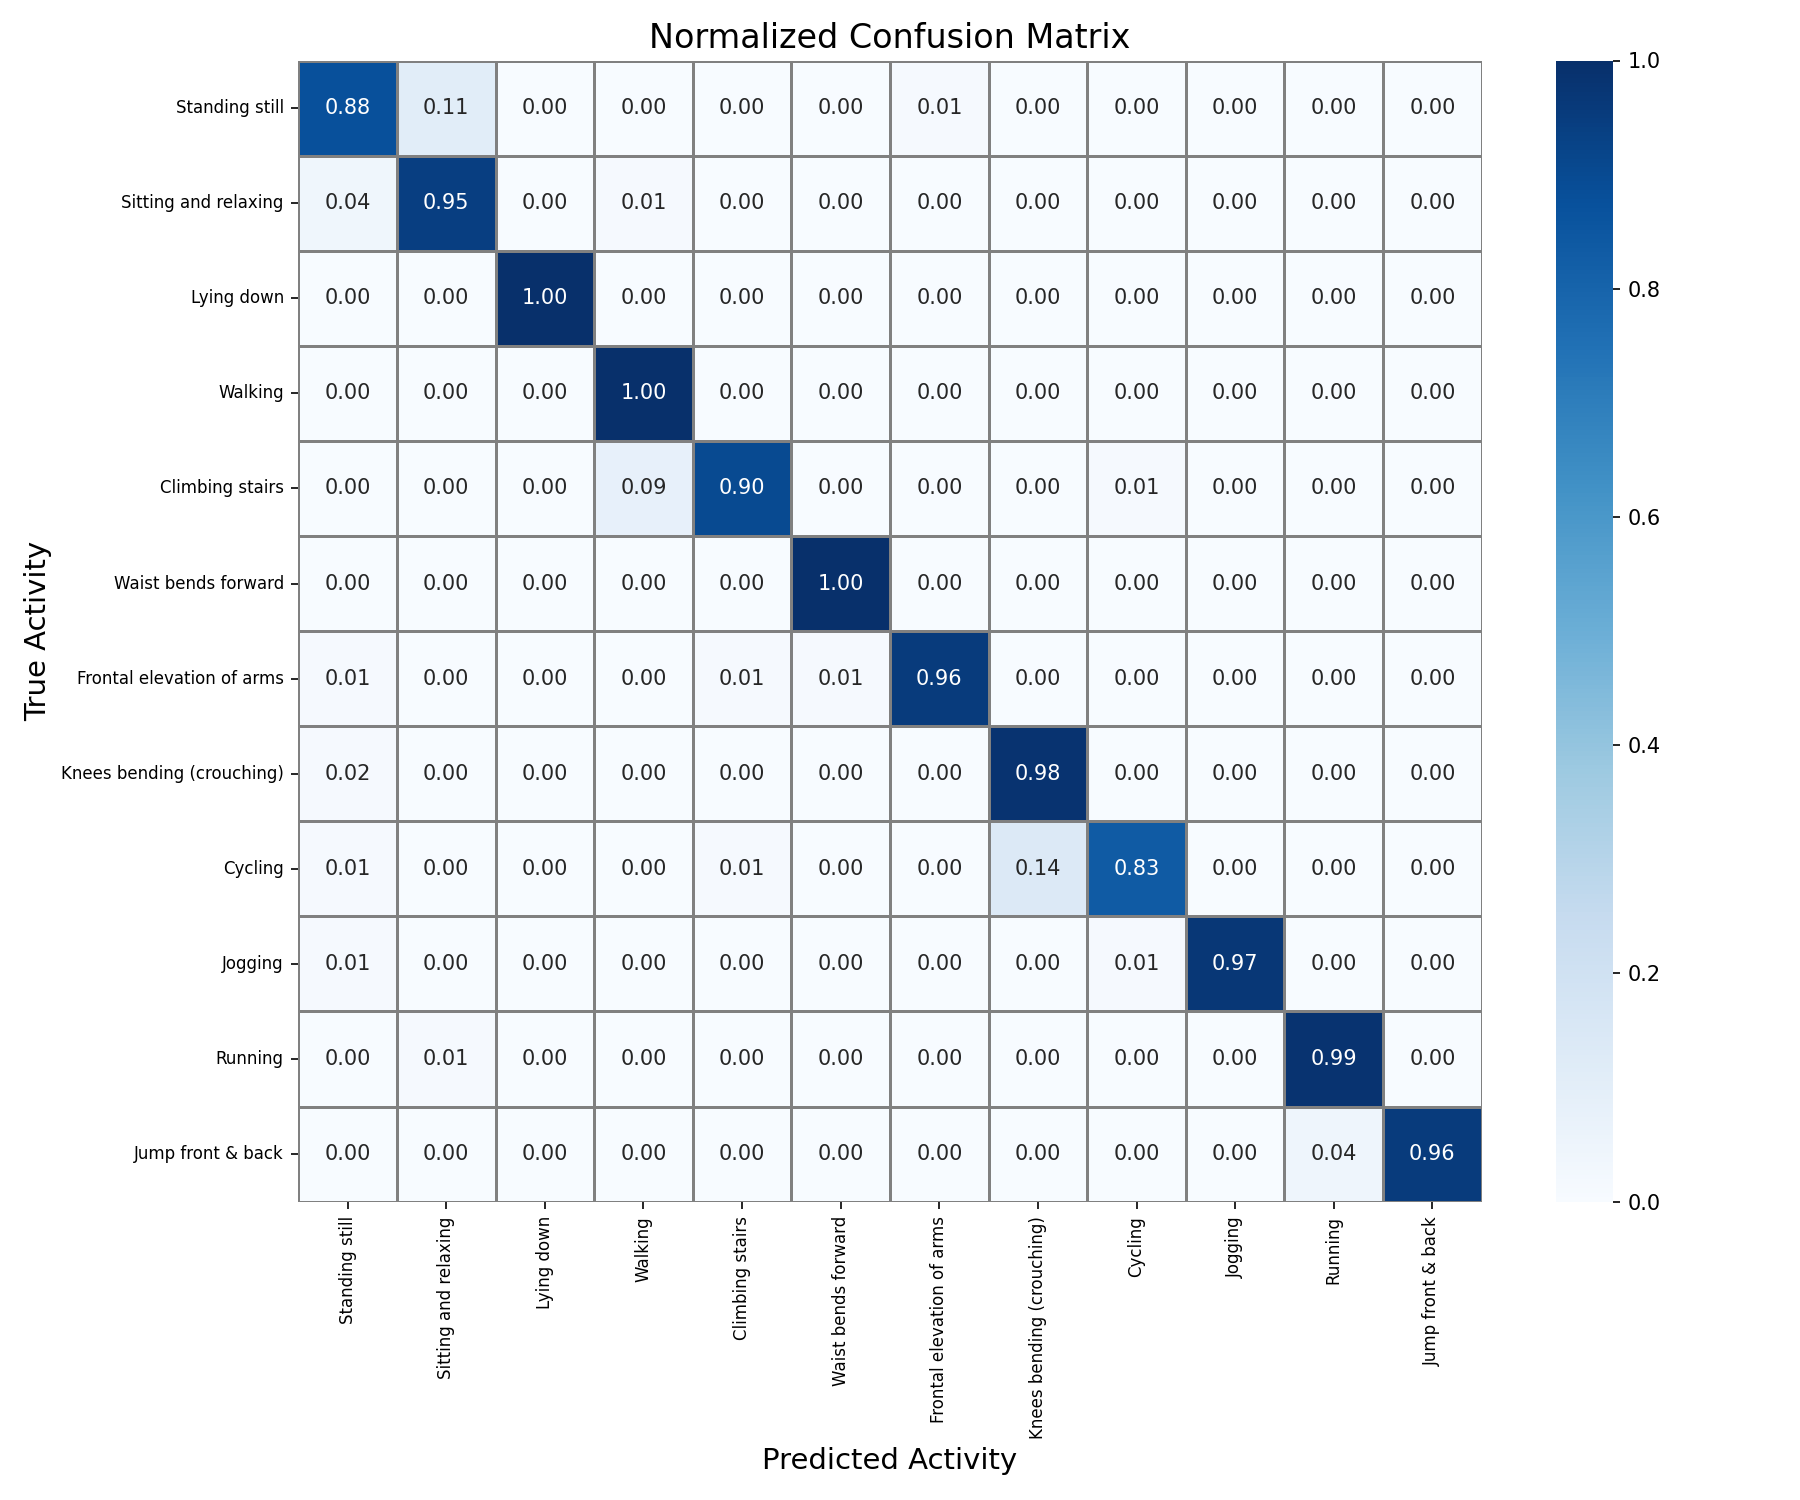
\includegraphics[width=\columnwidth]{figures/confusion_matrix.png}
\caption{Normalised confusion matrix for the 273-feature SVM model across 12 activities. Diagonal values close to 1.0 indicate accurate classification.}
\label{fig:cm}
\end{figure}

% ═══════════════════════════════════════════════
\section{Ablation Study}

\subsection{Motivation}
Multi-sensor HAR systems often include sensors at multiple body locations. However, additional sensors do not always improve performance --- they may introduce redundant or correlated features that expand the hypothesis space without adding discriminative information. We conduct a sensor-location ablation study to quantify each sensor's contribution.

\subsection{Experimental Setup}
Using a 252-feature baseline configuration (21 non-ECG channels $\times$ 12 features), we train four models: one with all sensors, and three with one sensor location removed at a time. Each experiment follows the same pipeline: load $\rightarrow$ preprocess $\rightarrow$ extract features $\rightarrow$ SMOTE $\rightarrow$ GridSearchCV $\rightarrow$ evaluate. A reduced grid ($C \in \{1, 10\}$, 3-fold CV) is used for computational efficiency.

\subsection{Results}
Table~\ref{tab:ablation} summarises the ablation results.

\begin{table}[H]
\centering
\caption{Sensor ablation results (252-feature baseline).}
\label{tab:ablation}
\small
\begin{tabular}{lccc}
\toprule
\textbf{Scenario} & \textbf{Acc.} & \textbf{Feats} & \textbf{$\Delta$} \\
\midrule
Baseline (all sensors) & 0.9124 & 252 & --- \\
Ablate chest (3 cols)  & 0.8883 & 216 & $-$2.64\% \\
Ablate arm (9 cols)    & 0.8959 & 144 & $-$1.81\% \\
Ablate ankle (9 cols)  & \textbf{0.9226} & 144 & $+$1.11\% \\
\bottomrule
\end{tabular}
\end{table}

\subsection{Analysis}

\textbf{Chest sensor (3 channels):} Removing the chest accelerometer causes the largest accuracy drop ($-$2.64\%). The chest sensor captures trunk orientation and is critical for distinguishing postures (standing vs.\ sitting vs.\ lying). Its three accelerometer channels encode the gravity-axis decomposition that separates these static classes.

\textbf{Arm sensor (9 channels):} Removing arm channels causes a 1.81\% drop. The arm sensor is important for upper-body activities (frontal arm elevation, waist bends) and provides complementary information to the chest sensor for activities involving arm movement.

\textbf{Ankle sensor (9 channels):} Removing the ankle sensor \textit{improves} accuracy by 1.11\%, from 91.24\% to 92.26\%. This counter-intuitive result suggests that the ankle features introduce more noise or redundancy than useful signal.

\subsection{Explaining the Ankle Redundancy}
Three factors explain why ankle removal helps:

\textbf{1.\ Multicollinearity.} Figure~\ref{fig:corr} shows the PCA-reduced correlation between ankle features (PC1) and other-sensor features (PC1). The high Pearson $R$ value indicates that the ankle sensor largely captures the same variance as the chest and arm sensors combined. This redundancy destabilises the SVM decision boundary.

\textbf{2.\ Dimensionality reduction.} Removing 108 ankle-derived features (from 252 to 144) shrinks the feature space by 43\%. For SVM, reducing redundant dimensions improves the margin and reduces overfitting in the dual space.

\textbf{3.\ Peripheral noise.} The ankle, being an extremity, is subject to greater movement artefacts from footwear, ground impact, and subject-specific gait idiosyncrasies. These patterns may not generalise across subjects.

\begin{figure}[H]
\centering
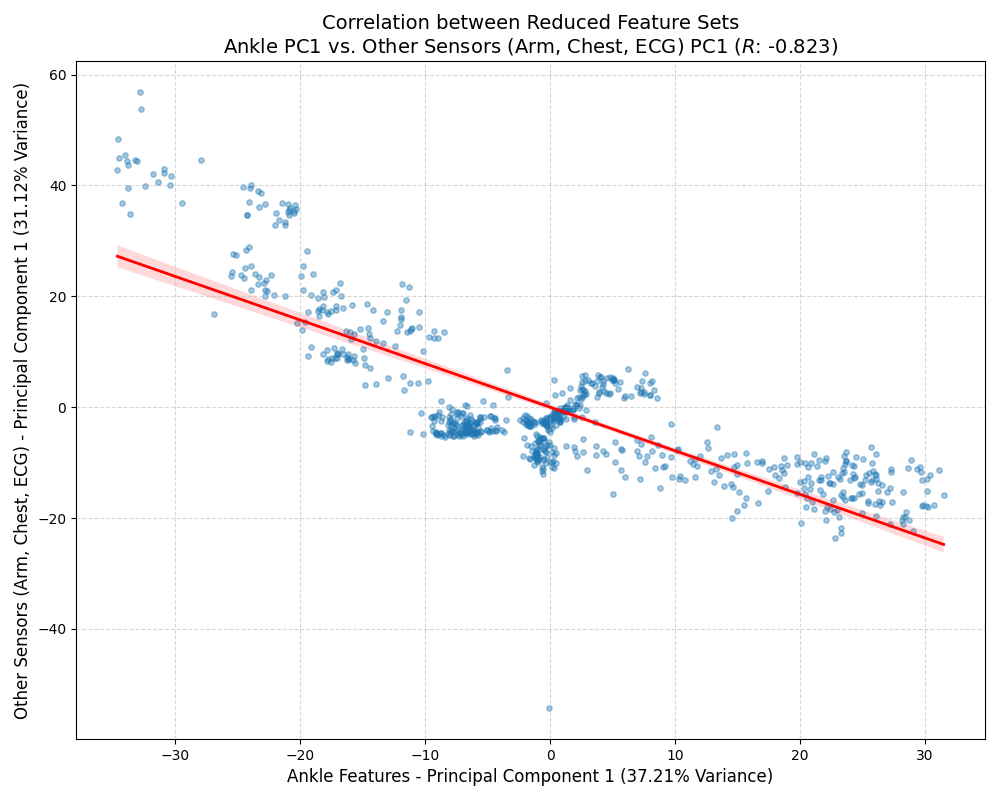
\includegraphics[width=\columnwidth]{figures/reduced_ankle_vs_others_correlation.png}
\caption{PCA correlation analysis: ankle features (PC1) vs.\ remaining sensor features (PC1). The high $R$ value demonstrates inter-sensor redundancy.}
\label{fig:corr}
\end{figure}

\textbf{Feature count discrepancy.} The main model (94.92\%, 273 features) differs from the ablation baseline (91.24\%, 252 features) due to a slightly different feature configuration. The ablation finding is valid as a controlled, within-experiment comparison.

% ═══════════════════════════════════════════════
\section{Reproducibility}

All experiments are fully reproducible. The GitHub repository\footnote{\url{https://github.com/Sourabh16/Human-Activity-Recognition-Using-Wearable-Sensors}} contains the complete source code, saved data split configuration, environment file (\texttt{requirements.txt}), final training logs, figure generation scripts, and exact reproduction commands. Key reproducibility measures include:

\begin{itemize}
    \item \textbf{Fixed random seed} (42) for SMOTE, SVM, and all stochastic operations.
    \item \textbf{Deterministic data split:} Subjects 1--7 for training, 8--10 for testing (hardcoded, no randomness).
    \item \textbf{Pinned dependencies:} All Python package versions are specified in \texttt{requirements.txt}.
    \item \textbf{Automated pipeline:} Three sequential scripts (\texttt{preprocessing.py} $\rightarrow$ \texttt{train.py} $\rightarrow$ \texttt{evaluate.py}) reproduce all results from raw data.
    \item \textbf{Checkpoints:} Model checkpoints ($<$2~MB) are regenerated deterministically and are not stored in version control.
\end{itemize}

The MHEALTH dataset is publicly available from the UCI Machine Learning Repository~\cite{banos2014mhealthdroid} and is not redistributed in the repository due to its size ($\sim$220~MB).

% ═══════════════════════════════════════════════
\section{Discussion}

\subsection{Comparison with Prior Work}
Table~\ref{tab:comparison} places our results in context with prior work on the MHEALTH dataset.

\begin{table}[H]
\centering
\caption{Comparison with published results on MHEALTH.}
\label{tab:comparison}
\small
\begin{tabular}{llc}
\toprule
\textbf{Method} & \textbf{Reference} & \textbf{Acc.} \\
\midrule
CNN + LSTM           & Ord{\'o}{\~n}ez \textit{et al.}~\cite{ordonez2016deep} & 91.0\% \\
SVM + 273 features   & \textbf{Ours}                                          & \textbf{94.9\%} \\
CNN-LSTM + Attention & Khatun \textit{et al.}~\cite{khatun2022deep}           & 98.8\% \\
\bottomrule
\end{tabular}
\end{table}

Our SVM pipeline outperforms the CNN+LSTM baseline by nearly 4 percentage points while using a fraction of the computational resources (CPU-only training in $\sim$10 minutes vs.\ GPU training over hours). The attention-based model achieves higher accuracy, but at the cost of interpretability and hardware requirements. For resource-constrained deployments (wearables, edge devices, clinical settings where model transparency matters), our approach offers a compelling accuracy--efficiency trade-off.

\subsection{Impact of Feature Design}
The success of our model hinges on the quality of the 273 engineered features. Time-domain features like mean and RMS capture postural information (gravity component, movement intensity), while frequency-domain features (FFT dominant frequency, PSD) capture rhythmic patterns crucial for distinguishing walking ($\sim$2~Hz) from jogging ($\sim$2.5~Hz) and running ($\sim$3~Hz). The zero-crossing rate provides a computationally cheap frequency proxy that is robust to signal amplitude variations.

Notably, the kurtosis and skewness features capture distributional shape --- these are important for activities with asymmetric motion profiles, such as ``waist bends forward'' (high skewness in the chest accelerometer y-axis) and ``jump front \& back'' (high kurtosis due to sharp impact peaks).

\subsection{Limitations}
Several limitations should be acknowledged. First, our window-level classification treats each 5.12-second segment independently, discarding temporal context that could help resolve ambiguous transitions. Second, the MHEALTH dataset contains only 10 subjects, which limits the statistical power of subject-independent evaluation. Third, our feature set is manually designed and may miss subtle discriminative patterns that representation learning could capture. Finally, the controlled laboratory setting of MHEALTH may not reflect the noise and variability of real-world deployments.

% ═══════════════════════════════════════════════
\section{Conclusion and Future Work}

This work demonstrates that the SVM with RBF kernel, combined with carefully engineered time-domain and frequency-domain features, achieves strong performance (94.92\% accuracy) on the MHEALTH HAR benchmark under subject-independent evaluation. The kernel trick enables the classifier to learn complex, non-linear activity boundaries without explicit feature space transformation.

The ablation study provides a key practical insight: more sensors and features do not always improve performance. The ankle sensor, despite providing 9 raw channels, introduced multicollinear features that degraded generalization. This finding has implications for wearable system design --- a two-sensor configuration (chest + arm) may be both cheaper and more accurate than a three-sensor setup.

\subsection{Future Work}
Several directions merit further investigation:

\textbf{Feature selection.} Applying Recursive Feature Elimination (RFE) or L1-based feature selection could systematically identify and remove redundant features across all sensor locations, potentially improving upon our 273-feature model. Mutual information-based selection could also reveal which of the 13 feature types contribute most to discriminability.

\textbf{Deep learning comparison.} A fair, controlled comparison between SVM and CNN/LSTM architectures on the same data split and evaluation protocol would quantify the accuracy--interpretability trade-off. Hybrid approaches that use handcrafted features as auxiliary inputs to deep networks are also worth exploring.

\textbf{Transfer learning and personalisation.} Our subject-independent protocol tests generalisation to entirely unseen users. In practice, a small calibration phase (5--10 labelled samples per activity from the target user) could be used for domain adaptation, potentially closing the gap to subject-dependent accuracy levels.

\textbf{Real-time deployment.} The trained SVM model is lightweight ($\sim$1.8~MB, $<$1~ms inference) and could be deployed on mobile or edge devices. Integrating the sliding-window feature extraction pipeline into a real-time streaming architecture (e.g., on Android Wear or a Raspberry Pi) is a natural next step for practical deployment.

\textbf{Activity transitions and temporal modelling.} Our current approach classifies each window independently, discarding temporal context. Incorporating sequence-level models such as Hidden Markov Models (HMMs) or Conditional Random Fields (CRFs) on top of SVM predictions could smooth out transient misclassifications and better handle transitions between activities.

\textbf{Sensor placement optimisation.} Our ablation study examined only complete sensor removal. A finer-grained analysis --- removing individual sensor \textit{types} (e.g., keeping ankle accelerometer but removing ankle gyroscope) --- could identify the minimal sensor configuration that preserves accuracy, reducing hardware cost and power consumption for wearable devices.

% ═══════════════════════════════════════════════
{\small
\bibliographystyle{ieee_fullname}
\begin{thebibliography}{10}

\bibitem{banos2014mhealthdroid}
O.~Banos, R.~Garcia, J.~A. Holgado-Terriza, M.~Damas, H.~Pomares, I.~Rojas, A.~Saez, and C.~Villalonga,
``mHealthDroid: a novel framework for agile development of mobile health applications,''
in \textit{Int.\ Workshop on Ambient Assisted Living}, pp.~91--98, Springer, 2014.

\bibitem{ordonez2016deep}
F.~J. Ord{\'o}{\~n}ez and D.~Roggen,
``Deep convolutional and LSTM recurrent neural networks for multimodal wearable activity recognition,''
\textit{Sensors}, vol.~16, no.~1, p.~115, 2016.

\bibitem{khatun2022deep}
M.~A. Khatun \textit{et al.},
``Deep CNN-LSTM with self-attention model for human activity recognition using wearable sensor,''
\textit{IEEE J.\ Transl.\ Eng.\ Health Med.}, vol.~10, pp.~1--16, 2022.

\bibitem{vapnik1995nature}
V.~Vapnik,
\textit{The Nature of Statistical Learning Theory}.
Springer, 1995.

\bibitem{scholkopf2002learning}
B.~Sch{\"o}lkopf and A.~J. Smola,
\textit{Learning with Kernels: Support Vector Machines, Regularization, Optimization, and Beyond}.
MIT Press, 2002.

\bibitem{bulling2014tutorial}
A.~Bulling, U.~Blanke, and B.~Schiele,
``A tutorial on human activity recognition using body-worn inertial sensors,''
\textit{ACM Computing Surveys}, vol.~46, no.~3, pp.~1--33, 2014.

\bibitem{bao2004activity}
L.~Bao and S.~S. Intille,
``Activity recognition from user-annotated acceleration data,''
in \textit{Pervasive Computing}, pp.~1--17, Springer, 2004.

\bibitem{anguita2013public}
D.~Anguita, A.~Ghio, L.~Oneto, X.~Parra, and J.~L. Reyes-Ortiz,
``A public domain dataset for human activity recognition using smartphones,''
in \textit{Proc.\ European Symposium on Artificial Neural Networks (ESANN)}, 2013.

\bibitem{chawla2002smote}
N.~V. Chawla, K.~W. Bowyer, L.~O. Hall, and W.~P. Kegelmeyer,
``SMOTE: Synthetic minority over-sampling technique,''
\textit{J.\ Artif.\ Intell.\ Res.}, vol.~16, pp.~321--357, 2002.

\bibitem{cortes1995support}
C.~Cortes and V.~Vapnik,
``Support-vector networks,''
\textit{Machine Learning}, vol.~20, no.~3, pp.~273--297, 1995.

\end{thebibliography}
}

\end{document}
